\documentclass{article}
\usepackage[utf8]{inputenc}
\usepackage{hyperref}
\usepackage[margin=12.7mm]{geometry}
\usepackage{helvet}
\usepackage{graphicx}
\usepackage{color}
\graphicspath{ {./UI/} }
\renewcommand{\familydefault}{\sfdefault}
\author{G12}
\title{Deals deTECHtor}
\date{}

\begin{document}
\maketitle
\tableofcontents
\clearpage
\section{Obiettivi del progetto}
Il progetto ha come obiettivo la realizzazione di un applicativo disponibile come app cross-platform (Android e IOS) in grado di ricercare prodotti
delle categorie tech negli e-commerce più famosi e permettere di tracciarne i prezzi.
Nello specifico questa app deve:
    \begin{itemize}
        \item Poter essere utilizzata sia senza account che con un account.
        \item Permettere di eseguire l’accesso tramite servizi come Google e Facebook
        \item Fornire la possibilità del recupero password di un account.
        \item Cercare prodotti sia per parola chiave che per categoria tech (Elettronica, Informatica, Software e Componentistica).
        \item Permettere di poter ordinare i prodotti per prezzo e per percentuale di sconto.
        \item Permettere di aggiungere/rimuovere prodotti ad una lista desideri, sincronizzata con l'account (se presente).
        \item Permettere di vedere il grafico prezzi di un prodotto.
        \item Permette di abilitare/disabilitare il tracciamento del prezzo di un prodotto nella lista desideri con notifiche
                in caso di cambiamenti via notifica push e/o e-mail (se presente).
        \item Dare la possibilità di visitare il sito e-commerce di un prodotto.
        \item Permettere di vedere l'affidabilità di un determinato sito e-commerce.
        \item Permettere di vedere la cronologia degli articoli visualizzati più recentemente.
    \end{itemize}
\section{Requisiti funzionali}
    \begin{itemize}
        \item L’applicazione deve essere a due livelli di accesso:
            \begin{enumerate}
                \item Utente anonimo
                \item Utente autenticato
            \end{enumerate}
        \item Funzionalità, con differenze tra tipi di utenti:
            \begin{enumerate}
                \item Alla prima apertura dell’app si apre la pagina di registrazione/login, una volta aggiunto un account non verrà più
                        richiesto di inserire tali informazioni. In questa pagina vengono chieste le informazioni necessarie per la
                        registrazione o il login. In basso alla pagina ci devono anche essere: il pulsante “accedi” nel caso in cui l’utente
                        abbia già un account, i pulsanti con i simboli di Google e Facebook per poter accedere con quei due servizi di terze
                        parti e la scritta “prosegui senza registrazione” o simile per proseguire con un account ospite.
                    \begin{itemize}
                        \item Account ospite: l’utente può direttamente utilizzare l’app. In questo caso la foto profilo sarà una foto profilo di
                                default e il nome utente sarà “guest”.
                        \item Registrazione con servizi di terze parti: premendo su uno dei due simboli dei servizi, l’app redirige l’utente alla
                                pagina di autenticazione. Nome utente e foto profilo vengono presi dai servizi.
                        \item Registrazione tradizionale: l'utente ha la possibilità di registrarsi inserendo la sua e-mail, una password e un
                                nome utente. Anche in questo caso la foto profilo sarà quella di default.
                        \item Login: se l'utente è già in possesso di un account, deve avere la possibilità di accedere tramite la sua e-mail
                                e password. L'utente deve anche avere la possibilità di recuperare la password.
                    \end{itemize}
                \item Ricerca prodotti: la ricerca può essere sia via parola chiave sia selezionando la categoria di interesse. Quando si
                        entra nella barra di ricerca, si può inserire la parola chiave e viene anche mostrata una lista delle categorie disponibili
                        (Elettronica, Informatica, Software, Componentistica). Viene mostrata una lista di prodotti che possono essere
                        ordinati sia per prezzo (default) che per percentuale di sconto, con un apposito selettore. Ogni articolo mostrato
                        deve avere le seguenti informazioni:
                \begin{itemize}
                    \item [a] Foto e nome.
                    \item [b] Prezzo.
                    \item [c] Percentuale di sconto (se presente).
                    \item [d] Affidabilità sito e-commerce.
                    \item [e] Se l’articolo è al suo minimo storico viene mostrata una stella prima del nome.
                \end{itemize}
                \item Dalla lista, selezionando un prodotto, l’utente può vedere il grafico di andamento del prezzo, salvarlo o eliminarlo
                (se già presente) nella lista desideri e visitare l’inserzione (viene aperta la pagina in questione in un browser in-app).
                \item Nella lista desideri:
                \begin{itemize}
                    \item [a] La lista desideri è una lista simile a quella dei prodotti nella finestra di ricerca, solo con alcune
                            funzionalità in più descritte nei prossimi punti e senza la barra di ricerca o la possibilità di ordinare
                            gli articoli (devono essere ordinati in base alla data di aggiunta).
                    \item [b] Selezionando un prodotto viene mostrata la stessa finestra del punto (3).
                    \item [c] Tenendo premuto un prodotto sarà possibile, tramite un menu:
                    \begin{itemize}
                        \item Abilitare le notifiche di abbassamento di prezzo. Si può decidere di ricevere una notifica se il prezzo
                                scende sotto un valore specificato dall’utente, in una apposita text box.
                        \item Selezionare la modalità di notifica che può essere tramite email (se utente autenticato), notifica push o entrambe.
                                Si possono selezionare i metodi di notifica solo se l'utente ha inserito un valore di soglia.
                    \end{itemize}
                \end{itemize}
                \item Nelle informazioni dell’account è possibile:
                \begin{itemize}
                    \item [a] Cambiare account
                    \item [b] Resettare la password.
                    \item [c] Impostare la foto profilo.
                    \item [d] Cambiare nome utente.
                    \item [e] Visualizzare la cronologia degli articoli visualizzati recentemente. Per definire un articolo come “visualizzato”
                    l’utente deve averlo selezionato dalla lista di ricerca prodotti. In questa pagina verrà mostrata una lista simile a quella
                    di ricerca ma solo con gli articoli visitati dall’utente (ordinati dal più recente). Dal momento che si vogliono visualizzare
                    solo quelli visualizzati più recentemente, articoli visualizzati più di 2 settimane prima non devono essere visualizzati.
                \end{itemize}
            \end{enumerate}
    \end{itemize}
\section{Requisiti non funzionali}
Compatibilità
\begin{enumerate}
    \item L’applicazione “Deals deTECHtor” deve essere un’app per Android (dalla versione 5.0) e IOS (dalla versione 8) per permeterne l'uso ad
        una platea più ampia di utenti.
    \item L’applicazione deve adattarsi ad ogni screen ratio per poter funzionare su qualsiasi tipo di dispositivo con tali OS poiché
            l’applicazione è pensata per funzionare non solo su smartphone ma anche su tablet, iPad, android TV.
    \item L’applicazione dovrà essere reperibile esclusivamente dagli store ufficiali apple e Google, per una questione di immagine e sicurezza.
\end{enumerate}
Lingua di sistema
\begin{enumerate}
    \item L’applicazione deve riconoscere la lingua del dispositivo, se essa è italiana l'applicazione sarà in italiano mentre se la lingua del
            dispositivo è una qualsiasi altra la lingua dell'applicazione sarà in inglese. Per permettere ad un più ampio bacino di utenti di utilizzare
            l'applicazione.
\end{enumerate}
Privacy
\begin{enumerate}
    \item Dai servizi di terze parti l’applicazione potrà solo prelevare le informazioni strettamente necessarie: foto profilo, email e nome utente.
            Questo per non richiedere informazioni che poi non verranno mai utilizzate e memorizzare inutilmente informazioni sensibili dell’utente.
    \item Al momento della registrazione/accesso l’utente deve essere avvisato che proseguendo andrà ad accettare i termini e condizioni di utilizzo
            e il trattamento dei dati personali.
    \item Se l’accesso viene eseguito tramite uno dei due servizi di terze parti (Google e Facebook) questi non devono essere poi collegati all’app,
            ma solo utilizzati per l’accesso. Non si vuole permettere ai servizi la raccolta di dati di utilizzo dell’app
\end{enumerate}
Scalabilità
\begin{enumerate}
    \item L’applicazione deve garantire la possibilità di gestione di un numero crescente di e-shops dal momento che sempre in crescita e si
            vuole mantenere la piattaforma aggiornata nel tempo. L’applicazione deve partire con la possibilità di gestire 20 e-shops,
            i top ranking, per poi prevedere di arrivare fino a 50 e-shops in futuro.
    \item L’applicazione deve prevedere un numero crescente di utenti. La quantizzazione di questo dato risulta difficile data la crescita
            molto veloce vista negli ultimi anni soprattutto con la pandemia l’utenza negli e-shops ha raggiunto velocità di crescita senza
            precedenti. Vedendo il numero di utenti che utilizzano servizi di tracciamento prezzi, ci si deve aspettare un bacino di almeno
            500000 utenti. La raggiunta del milione di utenti per un’applicazione di questo tipo è abbastanza remota in un futuro immediato
            quindi si può stare ben sotto a tale cifra nella progettazione. Il sistema, però, deve permettere in futuro una sua evoluzione e
            ampliamento senza dover svolgere cambiamenti drastici e molto costosi all’app.
\end{enumerate}
Sicurezza
\begin{enumerate}
    \item Registrazione tradizionale: per evitare errori di battitura l’utente deve inserire due volte l’indirizzo email (se sono diversi
        l’utente non può proseguire) e due volte la password (se sono diverse non può proseguire). Una volta inseriti i vari dati e confermata
        la registrazione deve essere inviata una e-mail con un link che permette all’utente di confermare la registrazione dell’account per
        assicurarsi che l'utente sia il vero possessore di quell'indirizzo e-mail.
    \item Login: l'utente accede semplicemente inserendo indirizzo e-mail e password. Come detto precedentemente, si deve dare la possibilità
        all'utente di recuperare la password in caso se la fosse dimenticata. La modalità di recupero password è: viene chiesto l’indirizzo
        e-mail e se corrispondente a un account esistente viene inviato un link per il recupero password. Premendo sul link ricevuto via
        e-mail viene aperta una pagina web dove si chiede all'utente di inserire due volte una nuova password che rispetti le caratteristiche
        descritte successivamente.
   \item Nel caso in cui venga effettuata la registrazione tradizionale, per motivi di sicurezza dell’account è richiesta una strong password.
        La password non deve essere uguale all’indirizzo email o al nome utente e deve essere maggiore di 8 caratteri e minore di 15 con
        almeno un numero e un simbolo.
   \item L'applicazione deve salvare le informazioni dell’account dell’utente in modo criptato per minimizzare la probabilità di violazione
        dell’account o l’accesso indesiderato ai dati personali dell’utente.
   \item Nel recupero password nella schermata di informazioni utente verrà chiesto all'utente di inserire la vecchia password e la nuova
        password due volte. La password deve rispettare i criteri già descritti. Verrà inviata una e-mail di notifica del cambiamento.
   \item {\color{red}I dati riguardanti l'utente devono essere salvati in modo cifrato. Questo per non esporre in chiaro le credenziali d'accesso e anche proteggere le informazioni dell'utente.}
\end{enumerate}
Prestazioni
\begin{enumerate}
    \item L’applicazione deve essere reattiva. L’avvio deve richiedere massimo 2 secondi e la navigazione tra i vari menu non deve richiedere più
            di 1 secondo. Inoltre, lo scrolling tra i prodotti non deve andare a scatti.
\end{enumerate}
Memorizzazione
\begin{enumerate}
    \item Al di fuori di un registro di log e dei file necessari per il suo funzionamento l’applicazione non deve memorizzare null'altro nel
            dispositivo su cui è installata.
   \item Dovrà essere salvata una lista con gli articoli visualizzati come descritto nel punto 5-e dei requisiti funzionali, questo però significa che solo i prodotti
        utili per la cronologia (visitati meno di 2 settimane fa) sono mantenuti in memoria, gli altri non devono essere salvati.
\end{enumerate}
Usabilità
\begin{enumerate}
    \item L’app deve essere user-friendly, le interfacce devono essere intuitive e le informazioni importanti devono subito essere viste
            dall’utente. Ad esempio, la stella davanti al nome di un prodotto il cui prezzo è al minimo storico deve essere ben visibile
            e distinguersi bene dal resto delle informazioni altrimenti l’utente si perde proprio le informazioni di cui più necessità.
            La pagina di registrazione e login deve essere il più chiara possibile, tutte le opzioni devono essere ben visibili. Quest’ultima
            va presa con molta attenzione, in un mondo in cui le app si installano e disinstallano con un click in mezzo secondo, la prima
            impressione è quella che conta davvero, difatti viene anche data la possibilità di utilizzare l’app senza un account proprio per
            renderla il più immediata possibile e non far perdere tempo all’utente frettoloso
\end{enumerate}
\section{Front-end}

Le immagini che saranno riportate successivamente sono state create solo per permettere una maggior chiarezza di  spiegazione. Non sono
un mockup o un modello da seguire in fase di design. Si deve anzi cercare di rendere  l’applicazione il più appetibile possibile con un
design interessante, che faccia insomma venire voglia di utilizzare  l’app, non asettico come le raffigurazioni riportate.
\begin{itemize}
        \item Deve essere chiaro all’utente dove si trova nell’applicazione, questo deve essere fatto con un indicatore (la linea blu delle
                foto che seguono) sopra al simbolo della schermata in cui si è.
        \item Schermata per la registrazione/login per il primo avvio: non ci sono vincoli particolari sulla realizzazione di  questa,
                basta che le funzionalità principali siano subito visibili e tutto rispetti le specifiche riportate sopra. 
                Sicuramente le icone per l’accesso con servizi di terze parti e il pulsante per continuare senza un account devono essere
                subito visibili perché sono quelle funzionalità che un nuovo utente andrebbe subito a cercare. Si può ad esempio mostrare una
                lista di opzioni per il login, che sia molto ordinata e chiara, e poi in base alla  scelta dell’utente si procederà con la
                richiesta delle informazioni necessarie in un’altra schermata. Come  detto precedentemente questa è la parte che deve essere
                più invogliante, essendo la prima cosa vista da un  nuovo utente.
        \item Come stato detto, per l’utilizzo dell’app l’utente deve accettare i rispettivi termini e condizioni e la normativa  della privacy.
                In questo caso sarebbe preferibile che, dopo che l’utente ha scelto il metodo di autenticazione,  si apra una finestra in cui viene
                detto che proseguendo l’utente accetta tali condizioni (con collegamento ai  termini cosicché l’utente possa facilmente consultarli).
                Questa finestra dovrà quindi avere due pulsanti, uno  per accettare e proseguire e uno per abortire la procedura di accesso o
                registrazione.
        \item Schermata principale / di ricerca prodotti:
        \begin{center}
                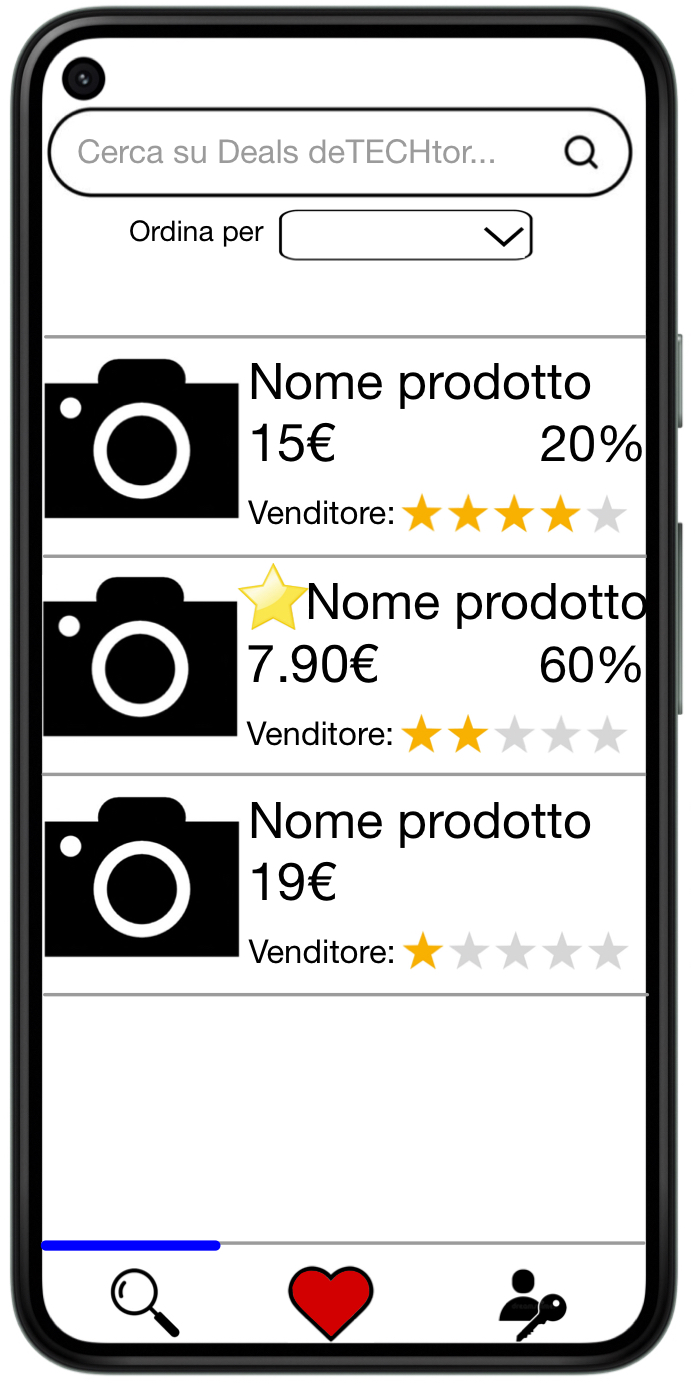
\includegraphics[width=40mm,scale=0.5]{ricerca.PNG}
        \end{center}
        \begin{itemize}
                \item In questa schermata ci devono essere tutti gli elementi descritti  
                          precedentemente, la barra di ricerca deve essere in alto, premendola deve essere  
                         quindi data la possibilità di inserire una parola chiave per la ricerca ma ci devono  
                         anche essere i 4 bottoni per la ricerca per categoria tech.
                \item La selezione dell’ordinamento non deve occupare molto spazio ma  
                         comunque essere visibile. A livello grafico per questa funzione non ci sono vincoli:  
                         drop-down menu, toggle-switch e radio buttons sono tutti elementi grafici che  
                         vanno bene.
                \item Come specificato, elementi importanti per l’utente come la stella per il  
                        minimo storico devono essere ben visibili, magari con un forte contrasto dal resto.
                \item Premendo su un prodotto si deve aprire una finestra dove l’utente potrà  
                         quindi controllare informazioni come il grafico dell’andamento del prezzo,  
                         aggiungere e rimuovere il prodotto dalla lista desideri magari con un pulsante a  
                         forma di cuore che è bianco quando il prodotto non è nella lista desideri e rosso  
                         quando lo è. Infine deve essere data la possibilità di aprire in un browser in-app la  
                         pagina del sito e-commerce corrispondente al prodotto che si sta visualizzando.      
        \end{itemize}
        \item Schermata lista desideri: la lista desideri deve essere simile a quella di ricerca ma con le differenze indicate  precedentemente.
                In questa schermata oltre alla risposta al tocco come nella schermata di ricerca, ci deve  anche essere la funzionalità della
                pressione prolungata, che aprirà una finestra con le varie funzionalità descritte precedentemente. Per  la selezione del metodo di notifica ci devono essere
                due pulsanti, uno raffigurante il simbolo di una lettera  (disabilitato per utente non autenticato) e uno il simbolo di un telefono e
                selezionando uno o entrambi si  abiliteranno le notifiche con i metodi selezionati.Come detto prima si possono selezionare i
                metodi di notifica solo se l'utente ha già inserito il valore di soglia nell'apposita text box. Bisogna rendere evidente
                all'utente che prima deve mettere quel valore e poi selezionare i metodi di notifica quindi la text box deve essere ben
                visibile Ovviamente quando si è in questa schermata l’indicatore  blu deve essere sopra al cuore.
        \item Questa è la schermata un po’ più semplice e con meno funzionalità. Deve solo  essere chiaro all’utente che premendo sul nome
                utente e sulla foto questi  possono essere modificati, per questo fine si possono usare dei simboli di  modifica come
                raffigurato. Avendo poche funzionalità questa schermata deve  essere semplice ed immediata.
        \begin{center}
                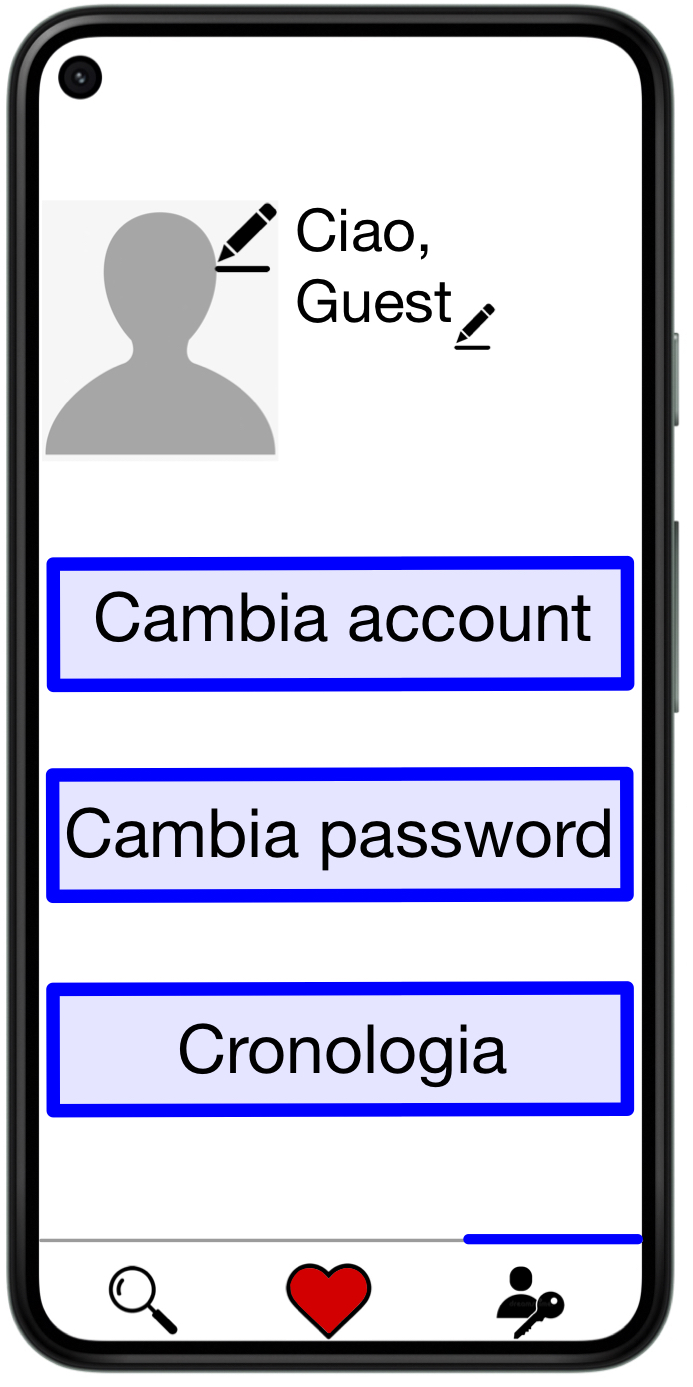
\includegraphics[width=40mm,scale=0.5]{area personale.PNG}
        \end{center}
\end{itemize}
\section{Back-end}
\begin{itemize}
    \item L’applicazione deve utilizzare le APIs dei vari siti e-commerce per ricevere la lista dei prodotti cercati.
    \item {\color{red}Per il tracking dei prezzi l'applicazione deve utilizzare le APIs fornite dai siti e-commerce}. 
    \item L'applicazione dovrà supportare l’autenticazione utente tramite servizi di terze parti (Google e Facebook) grazie alle loro APIs.
    \item L’applicazione deve utilizzare il servizio del sistema operativo del dispositivo su cui è installata per inviare notifiche push.
    \item Per identificare l’affidabilità di un sito di e-commerce ci si deve affidare alle APIs della piattaforma Trustpilot.
    \item Per il browser in-app che permette di visitare il sito e-commerce di un prodotto ci si può appoggiare a IIAB che fornisce una
            semplice API con la quale si possono creare browser in-app. Per questo tipo di app non serve un’esperienza di navigazione avanzata,
            quindi una API come questa è sufficiente permettendo una navigazione link-driven e con semplici funzionalità come andare avanti e
            indietro, condividere la pagina visitata e chiudere in qualsiasi momento il browser per tornare all’app.
    \item {\color{red}I dati riguardanti gli account degli utenti (inclusa la lista desideri) devono essere salvati in un database esterno.}
\end{itemize}
\begin{center}
        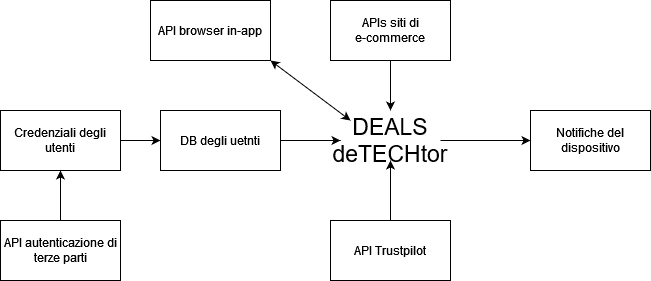
\includegraphics[width=130mm]{diagramma.png}
\end{center}
\section{Sintesi discussione con gruppo abbinato (G11)}
Preme precisare che le modifiche sono state davvero poche dal momento che il documento in fin dei conti è risultato chiaro e senza punti ambigui. Abbiamo comunque
apportato delle modifiche per rendere ancora meno fraintendibile ciò che era stato scritto.\\
Gli obbiettivi e i requisiti funzionali sono rimasti completamente invariati.\\
È stata apportata una modifica ai requisiti non funzionali. Il punto 6 della sicurezza è stato riscritto completamente. La modifica è stata una decisione presa
direttamente da noi, questo perché era stato scritto in modo ambiguo e assolutamente poco chiaro. Non avevamo notato tale errore controllando il documento prima di
consegnarlo ed esporlo al gruppo abbinato.\\
Per quanto riguarda il back-end sono state apportate due modifiche:
\begin{enumerate}
        \item Il secondo punto è stato riscritto perché poco chiaro ma il contenuto è rimasto invariato.
        \item È stato aggiunto un punto per specificare che i dati degli account degli utenti dovranno essere salvati in un database. Lo avevamo già inserito nello
                schema ma è stato preferito scriverlo esplicitamente per rendere meno ambiguo dove dovessero essere salvate tali informazioni.
\end{enumerate}
Abbiamo ricevuto l'OK dal gruppo abbinato (G11) per le modifiche apportate il giorno 01/10/2021 perciò questo è il documento finale accordato tra le parti.
\end{document}